\icode[magenta]{E-MI-MU-L4-261104-001}
（多选）
如图所示，三根轻质细线结于\(O\)点，\(OA\)另一端固定在天花板上的\(A\)点（位于圆心\(O^{\prime}\)的正上方），\(OB\)另一端连接质量为\(m\)的小球\(P\)（可视为质点），\(OC\)另一端连接质量为\(2m\)的物体\(Q\)，将小球\(P\)放置于半径为\(R\)、质量为\(3m\)的圆表面光滑的半圆柱上,半圆柱及物体\(Q\)均放置于粗糙水平面上，当\(A\)、\(O\)、\(O^{\prime}\)处于同一竖直线上时，\(OC\)处于水平且物体\(Q\)恰好不滑动，此时\(OB = \frac{3}{2}R\)，\(OO^{\prime} = 2R\)，重力加速度大小为\(g\)，最大静摩擦力等于滑动摩擦力，则下列说法正确的是\paren[]

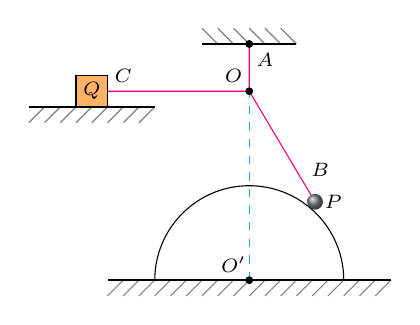
\begin{tikzpicture}[font=\scriptsize]
	\draw[dashed,cyan] (0,0)--(0,2.4);
	\draw (1.2,0) arc(0:180:1.2);
    \draw[magenta] (50:1.3)--(0,2.4)--(-1.8,2.4) (0,3)--(0,2.4);
	\draw[fill=orange!60] (-1.8,2.2) rectangle(-2.2,2.6)node[midway]{\(Q\)};
	\shade[ball color=gray] (50:1.3)node[right]{\(P\)} circle(.1);
	\foreach \x in {-2.8,-2.6,...,-1.4}
		\draw[gray] (\x,2)--++(.2,.2);
	\foreach \x in {-1.8,-1.6,...,1.6}
		\draw[gray] (\x,-.2)--++(.2,.2);
	\foreach \x in {-.6,-.4,...,.6}
		\draw[gray] (\x,3.2)--++(.2,-.2);
	\draw[thick] (-1.8,0)--(1.8,0) (-.6,3)--(.6,3) (-2.8,2.2)--(-1.2,2.2);
	\fill (0,2.4) circle(.05) (0,0) circle(.05) (0,3) circle(.05);
	\node at(.2,2.8){\(A\)};
	\node at(-.2,.2){\(O^{\prime}\)};
	\node at(-.2,2.6){\(O\)};
	\node at(.9,1.4){\(B\)};
	\node at(-1.6,2.6){\(C\)};
\end{tikzpicture}
\begin{choices}
	\item 半圆柱所受的摩擦力与物体\(Q\)所受到的摩擦力大小相等
	\item\(OC\)段绳子的拉力大小为\(\frac{3 \sqrt{15}}{16}mg\)
	\item 水平面对圆柱体的支持力大小为\(4mg\)
	\item 物体\(Q\)与水平面间的动摩擦因数为\(\frac{3 \sqrt{15}}{64}\)
\end{choices}
\begin{answer}
	AD\qquad 提示：
\end{answer}